\chapter{Introduction}

Agricultural production system is an outcome of a complex interaction of seed, soil, water and agro-chemicals (including fertilizers). Therefore, judicious management of all the inputs is essential for the sustainability of such a complex system. The focus on enhancing the productivity during the Green Revolution coupled with total disregard of proper management of inputs and without considering the ecological impacts, has resulted into environmental degradation. The only alternative left to enhance productivity in a sustainable manner from the limited natural resources at the disposal, without any adverse consequences, is by maximizing the resource input use efficiency. It is also certain that even in developing countries, availability of labour for agricultural activities is going to be in short supply in future. The time has now arrived to exploit all the modern tools available by bringing information technology and agricultural science together for improved economic and environmentally sustainable crop production. Precision agriculture merges the new technologies borne of the information age with a mature agricultural industry. It is an integrated crop management system that attempts to match the kind and amount of inputs with the actual crop needs for small areas within a farm field. This goal is not new, but new technologies now available allow the concept of precision agriculture to be realized in a practical production setting.

Many technological developments occurred in the last decade that has improvised the concept of Precision Farming (PF). Precision agriculture (PA) or satellite farming or site specific crop management (SSCM) is a farming management concept based on observing, measuring and responding to inter and intra-field variability in crops.~\cite{mcbratney2005future,whelan2003definition} The goal of precision agriculture research is to define a decision support system (DSS) for whole farm management with the goal of optimizing returns on inputs while preserving resources. The adaptability of this technique relies on the integration and utilisation of modern days technologies such new advance farm technologies with the single system site specific technologies. The technology varies from high speed connectivity of internet, farmer awareness. PF is an integrated, information and agricultural management system that is designed to improve the whole farm production efficiency with the low cost effect while avoiding the unwanted effects of chemical loading to the environment. The focus under PF is to gather information regarding the soil and crop condition and capture the sequence on the soil and crop conditions at spatial level.

\section{Motivation}

Precision agriculture means application of precise and correct amount of inputs like water, fertilizer, pesticides etc. at the correct time to the crop for increasing its productivity and maximizing its yields. Precision agriculture management practices can significantly reduce the amount of nutrient and other crop inputs used while boosting yields. Farmers thus obtain a return on their investment by saving on phytosanitary and fertilizer costs. The second, larger scale benefit of targeting inputs in spatial, temporal and quantitative terms concerns environmental impacts. Applying the right amount of inputs in the right place and at the right time benefits crops, soils and groundwater, and thus the entire crop cycle. Consequently, precision agriculture has become a cornerstone of sustainable agriculture, since it respects crops, soils and farmers. Sustainable agriculture seeks to assure a continued supply of food within the ecological, economic and social limits required to sustain production in the long term. Precision agriculture therefore seeks to use high-tech systems in pursuit of this goal. 

In a developing country like India the use of precision farming can help to boost the economic growth in agriculture via substantial increase in crop yield. The overall cost and infrastructure needed to meet this goal still seems a challenging task to be accomplished. We therefore decided to build an end-to-end solution for precision farming by building a low cost system. 

\section{System Overview}
We aim to design a low cost system to solve the problems discussed above and help the farmers gain better insights of the farms. A flowchart of the system is shown in Fig.~\ref{fig: extra-1}. The system consists of image capturing of the farm by the drone. These images are then uploaded on the server for image processing and analysis. The analyzed image is  overlaid on Google Maps for better visualization of the farm showing critical areas in different colors. The photographs of the critical areas can be uploaded on our applictaion to be evaluated for prescription of crop diseases.
\begin{figure}[!h]
	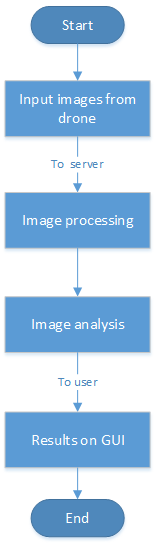
\includegraphics[height=0.9\linewidth]{extra-1}
	\centering
	\caption{\label{fig: extra-1}Flowchart of the System Workflow}
\end{figure}.


\section{Objectives}

The main objectives of the project are:

\begin{itemize}
	\item Build a low cost drone with the use of a flight controller having the functionality of stable and autonomous flight. (having capability of hovering and following the flight of guided waypoints)
	\item Perform image processing to stitch the images using Open Drone Map
	\item Perform image analysis with two approaches i.e. Vegetation 	Index(VI) methods and machine learning on hyperspectral data, and deep learning on RGB data.
	\item Build a Graphical User Interface(GUI) and an Android Application.
\end{itemize}


\section{Structure of the document}
The report is divided into five chapters with each part describing different aspects of the project. The second chapter presents a literature survey on the knowledge obtained on the topic. The third chapter describes the methods and tools used to build/assemble the drone required for above mentioned functionality. The fourth chapter provides insights into the image processing techniques applied to achieve the best results. The fifth chapter describes the methods used for image analysis. The sixth chapter deals with the development of the GUI for the end user clients.


